\section{Algorithms\label{sec:algo}}

We now detail a set of algorithms to solve the integral equation in \cref{eq:int-eq} and evaluate the solution via the double layer integral in \cref{eq:double_layer} at a given target point $\vx \in \Omega$.
As described in the previous section, both solving \cref{eq:int-eq} and evaluating \cref{eq:double_layer} require accurate evaluation of singular/near-singular integrals of functions defined on the surface $\Gammah$.
We first outline our unified singular/near-singular integration scheme, \qbkix, its relation to existing approximation-based quadrature methods and geometric problems that can impede accurate solution evaluation.
We then describe two geometry preprocessing algorithms, \textit{admissibility refinement} and \textit{adaptive upsampling}, that address these issues to obtain the sets of patches $\Pcoarse$ and $\Pfine$ used by \qbkix.

\subsection{Singular and Near-Singular Evaluation \label{sec:singular-eval}}
%We start with describing our (near-) singular integration algorithm, identifying conditions that the patches need to satisfy for the algorithm to achieve a target accuracy $\etrg$.

%We start with the informal idea of the algorithm. As in all QBX-style algorithms, we take advantage of the fact that while the integrand may be (near-)singular, the solution of the PDE given by the integral is not, and can be extrapolated from points where it can be computed reliably to points close to the surface or on the surface. 
We begin with an outline of the algorithm.
%As with all \qbx-style algorithms, we observe that while the integrand may be singular/near-singular for a particular choice of $\vx$, the solution of the PDE given by \cref{eq:double_layer} is well-defined. 
%This allows us to extrapolate the solution to $\vx$ from nearby points where the integrand is smooth and standard quadrature rules are accurate.
%Specifically, for a quadrature sample $x_j$ on a patch $P$ from $\Pcoarse$, where we need to evaluate the singular integral  to solve \cref{eq:int-eq}, we compute the values for extrapolation at points $c_{j,s}$ (check points) sampled along the normal to the surface at $\vy_j$.  Suppose we fix the placement of points $c_{j,s}$ in the interior of $\Omega$.  We can always refine $\Pfine$  so for evaluation of integrals at these points $c_{j,s}$ the smooth quadrature rules using denser quadrature points $\tilde{x}_j$  on $\Pfine$ are sufficiently accurate. Then extrapolation to $\vy_j$ can be applied to these accurate values.  In practice, we perform refinement to obtain  $\Pcoarse$,  not just $\Pfine$ (admissibility refinement). For $\Pcoarse$, we use a heuristic error estimate to place check points for every $x_j$,  and refine patches to ensure that they are away from patches other than $P$. In this way, the amount of refinement needed for $\Pfine$ is reduced.  
For a point $\vsx \in \Gammah$ on a patch $\vP$ from $\Pcoarse$ that is closest to $\vx$, we first upsample the density $\phi$ from $\Pcoarse$ to $\Pfine$ and compute the solution at a set of points $\vc_s$, $s = 1, \hdots p$ called \emph{check points}, sampled along the surface normal at $\vsx$ away from $\Gammah$. 
We use \cref{eq:double_layer_disc} to approximate the solution at the check points.
We then extrapolate the solution to $\vx$.
%The placement of check points relative to $\Pcoarse$ is critical to ensuring the accuracy of the overall method. 
%In \cref{sec:admissible}, we list the geometric criteria that $\Pcoarse$ must satisfy in order to solve \cref{eq:int-eq} accurately; we enforce these criteria by a sequence of quadrisection algorithms called \emph{admissibility refinement}. 
%The resulting set of patches determines a set of check points $\{\vc_{I,s}\}$ in $\Omega$, which are used to extrapolate the solution to each of the quadrature samples $\vy_I$ in the discretization of $\Pcoarse$.
%Once we fix a set of check points, we further refine $\Pcoarse$ to produce a set of patches $\Pfine$ such that \cref{eq:double_layer_disc} can be evaluated accurately at each $\vc_{I,s}$. 
%The algorithm to construct $\Pfine$ from $\Pcoarse$ is called \emph{adaptive upsampling}.
%We use empirical heuristics to place check points in admissibility refinement and trigger refinement in adaptive upsampling to reduce the overall amount number of quadrature patches in $\Pfine$.


For a given surface or quadrature patch $\vP: \I^2 \rightarrow \mathbb{R}^3$,  we define the \textit{characteristic length} $L(P)$ as the square root of the surface area of $\vP$, i.e., $L(\vP) = \sqrt{\int_{\vP}d\vy_{\vP}}$.
We use  $L = L(\vP)$ or $L_\vy$ for $\vy \in \vP(D)$ to denote the characteristic length when $\vP$ is clear from context.
For a point $\vx \in \Omega$, we assume that there is a single closest point $\vsx \in \Gammah$ to $\vx$; all points to which the algorithm is applied will have this property by construction.  
Note that $\vn(\vsx)$, the vector normal to $\Gammah$ at $\vsx$, is chosen to point outside of $\Omega$.
%We assume that two sets of patches are defined:  $\Pcoarse$, which serves as the discretization of $\Gamma$, and $\Pfine$, which is obtained from $\Pcoarse$ by refinement.
%We will provide a detailed discussion regarding this refinement in \cref{sec:adaptive_upsampling}.

%Expanding \cref{eq:double_layer_disc}, we obtain the following approximation of $u$ with respect
%to discretization on a collection of patches $\qP$:
%\begin{equation}
%  \hat{u}(\vx; \qP) = \sum_{P \in \qP}\sum_{\ell \in I(P)} \frac{\partial G(\vx,\vy_\ell)}{\partial n}\cdot \phi_\ell w_\ell.
%\label{eq:double_layer_disc}
%\end{equation}
%We want to compute $\hat{u}$ such that $\|u(\vx) - \hat{u}(\vx)\|_2 \leq \etrg$.

%Recall \cref{eq:double_layer_disc}, in which we defined $\hat{u}(\vx;\Pcoarse)$ as the discretization of \cref{eq:double_layer} with a quadrature rule for smooth funcitons. 
%\edittxt{We define three zones in $\Omega$, in terms of \cref{eq:double_layer_disc}, for which \cref{eq:double_layer} is evaluated differently.}{We define three zones in $\Omega$ for which \cref{eq:double_layer} is evaluated differently in terms of \cref{eq:double_layer_disc} and the desired solution accuracy $\etrg$ .}
We define three zones in $\Omega$ for which \cref{eq:double_layer} is evaluated differently in terms of \cref{eq:double_layer_disc} and the desired solution accuracy $\etrg$ .
The \emph{far field}  $\Omega_F = \{\vx \in \Omega \,|\, \|u(\vx) - \hat{u}(\vx;\Pcoarse)\|_2 \leq \etrg\}$, where the quadrature rule corresponding to $\Pcoarse$ is sufficiently accurate, and the \emph{intermediate field}  $\Omega_I= \{\vx \in \Omega \,|\, \|u(\vx) - \hat{u}(\vx;\Pfine)\|_2 \leq \etrg\}$, where quadrature over $\Pfine$ is sufficiently accurate.
The remainder of $\Omega$ is the \emph{near field} $\Omega_N = \Omega \setminus \Omega_I$.

%In a large portion of $\Omega$, computing $\hat{u}(\vx, \Pcoarse)$ or $\hat{u}(\vx, \Pfine)$ with \cref{eq:double_layer_disc} directly is sufficient.

%We'll refer to $\Omega_F$ as the \textit{far field} of $\Pcoarse$ and $\Omega_I$ as the \textit{intermediate field} of $\Pcoarse$.

%When $\vx$ is not in $\Omega_I$, special treatment is required to approximate the potential.

\paragraph*{Non-singular integration}
To compute the solution at points $\vx$ in $\Omega_F$, \cref{eq:double_layer_disc} is accurate to $\etrg$, so we can simply compute $\hat{u}(\vx, \Pcoarse)$ directly.
Similarly for points in $\Omega_I \setminus \Omega_F$, we know by definition that $\hat{u}(\vx, \Pfine)$ is sufficiently accurate, so it can also be applied directly. 

\paragraph*{Singular/near-singular integration algorithm}


\begin{figure}[!htb]
  %\setlength\figureheight{1.9in}
  %\setlength\figurewidth{2.1in}
  \begin{minipage}{\textwidth}
  \centering
      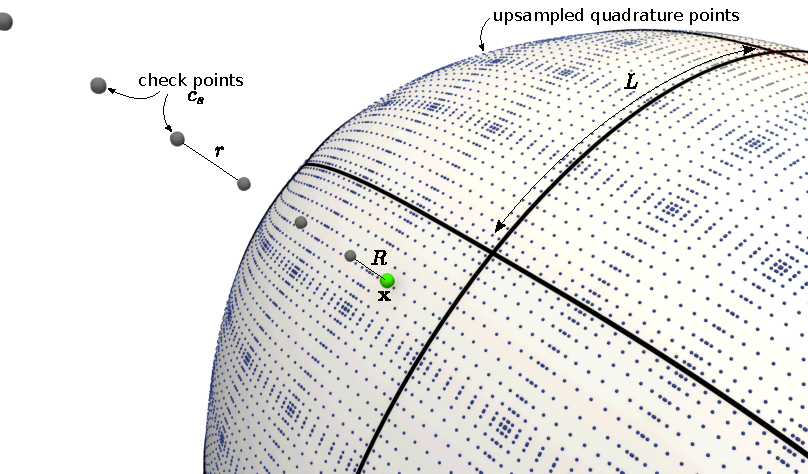
\includegraphics[width=.85\linewidth]{figs/qbkix_schematic.pdf}
  \end{minipage}\hfill
  \mcaption{fig:qbkix-schematic}{Schematic of singular/near-singular
  evaluation}{A small piece of a boundary $\Gammah$ is shown, along with the set of
  patches $\Pcoarse$ (patch boundaries are drawn in black). The target point $\vx$, in this
  case on $\Gammah$, is shown in green. The solution is evaluated
  at the check points $\vc_s$ (gray points off-surface) using the fine
  discretization $\Pfine$ (small dots on-surface). The distance from the first
  check point $\vc_0$ to $\Gammah$ is $R$ and the distance between consecutive
  check points $\vc_i$ and $\vc_{i+1}$ is $r$. In this example, $\Pfine$ is computed
  from $\Pcoarse$ with two levels of uniform quadrisection, producing 16 times
  more patches. The patch length $L$ is roughly proportional to the average edge
  length of the patch.}
\end{figure}

For the remaining points in $\Omega_N$, we need an alternative means of evaluating the solution.
In the spirit of the near-singular evaluation method of \cite{YBZ},  we construct a set of \textit{check points} $\vc_0, \hdots, \vc_p$ in $\Omega_I$ along a line intersecting $\vx$ to approximate the solution near $\vx$. 
However, instead of interpolating the solution as in \cite{YBZ}, we instead extrapolate the solution from the check points to $\vx$.
%We first place check points in $\Omega_I$, compute $\hat{u}(\vc_i, \Pfine)$ for each $i$, then extrapolate the approximate values at the check points to $\vx$.  \note[MJM]{kill sentence}
We define two distances relative to $\vsx$: $R(\vsx) =b L_\vsx = \|\vc_0 - \vsx\|_2$, the distance from the first check point $\vc_0$ to $\Gammah$,  and $r(\vsx) =a L_\vsx = \|\vc_i - \vc_{i+1}\|_2$, the distance between consecutive check points.
We assume  $0<a,b <1$.
%The points are placed along the surface normal $\vn(\vsx)$. 

The overall algorithm for the unified singular/near-singular evaluation scheme is as follows.
A schematic for \qbkix is depicted in \Cref{fig:qbkix-schematic}.


\begin{enumerate}
  \item Find the closest point $\vsx$ on $\Gammah$ to $\vx$.
  \item Given values $a$ and $b$, generate check points $C = \{\vc_0, \hdots, \vc_{p}\}$ 
    %distance $R(\vy)$ away from the $\Gamma$ and equispaced in $\vr(\vy)$ along the inward-pointing normal:
    \begin{equation}
      \vc_s = \vsx -(R(\vsx) +s r(\vsx)) \vn(\vsx), \quad s=0, \hdots, p
      \label{eq:check}
    \end{equation}
    The center of mass of these check points $\vhc$ is called the \textit{check center} for $\vx$.
    Note that $\Pfine$ must satisfy the condition that $\vc_s$ are in $\Omega_I$ for a given choice of $a$ and $b$.
\item Upsample $\phi$. 
  We interpolate the density values $\phi_I$ at $x_I$ on patches in $\Pcoarse$ to quadrature points $\tilde{x}_J$ on patches in $\Pfine$ 
  with global indices $I$ and $J$ on $\Pcoarse$ and $\Pfine$ respectively.
  If a patch $\vP_i$ in $\Pcoarse$ is split into $m_i$ patches in $\Pfine$, we are interpolating from $q^2$ points to $m_iq^2$ points.
  %Let $\wfine$ and $\phifine$ be the vector quadrature weights and interpolated density values at $\tilde{x}_J$ of $\Pfine$.
  \item Evaluate the potential at check points via smooth quadrature with the upsampled density, i.e. evaluate $\hat{u}(\vc_s) = \hat{u}(\vc_s, \Pfine)$ for $s=0,\hdots, p$.
  \item Compute a Lagrange interpolant $\tilde{u}$ through the check points $\vc_0,\hdots, \vc_p$ and values $\hat{u}(\vc_0), \hdots, \hat{u}(\vc_{p})$ and evaluate at the interpolant at $\vx$:
      \begin{equation}
          \tilde{u}(\vx) = \sum_{s=0}^p \hat{u}(\vc_s)\ell_s(t_\vx),
      \end{equation}
        where $\ell_s(\vx)$ is the $s$th Lagrange basis function through the points $\vc_0,\hdots, \vc_p$, and $t_\vx\in \mathbb{R}$ is such that $\vx = \vsx - t_\vx\vn(\vsx)$ (see \cref{fig:extrap-err-setup} for a schematic of the check points).
    Since $\vx$ lies between $\vc_0$ and $\Gammah$, we are extrapolating when computing $\tilde{u}(\vx)$.
\end{enumerate}

%\begin{algorithm}
%    \KwData{A set of surface patches $\Pcoarse$, a set of quadrature patches $\qPfine$, a target point $\vx$, extrapolation order $p$, quadrature order $q$, }
%  \KwResult{The closest point $\vsx$ on $\qP$ to $\vx$}
%
%  \DontPrintSemicolon
%  Construct an AABB tree $T_T$ from a fine triangle mesh of the quadrature patches of $\qP$\;
%  Construct an AABB tree $T_B$ from bounding boxes of quadrature patches in $\qP$.\;
%    $\tau_0 = $ closest triangle to $\vx$ computed with $T_T$ \;
%  
%    $P_{i_0} = $ patch corresponding to $\tau_0$\;
%    Find the closest point $\vector{s}_{\vector{\vx},0}$ on $P_{i_0}$ to $\vx$ with \cref{app:closest_point}.\;
%    $d_{i_0} = \|\vx - \vector{s}_{\vector{\vx},0}\|_2$\;
%    $B_{d_{i_0}}(\vx)=$ a box centered a $\vx$ with edge length $2d_{i_0}$\;
%    Find the boxes $B_{i_1}, \hdots B_{i_k}$ in $T_B$ that intersect $B_{d_{i_0}}(\vx)$\;
%    
%    \For{$B_{i_j} \in B_{i_1}, \hdots B_{i_k}$}{
%      $P_{i_j} =$ quadrature patch corresponding to $B_{i_j}$ \;
%      Find the closest point $\vector{s}_{\vector{\vx},j}$ on $P_{i_j}$ to $\vx$ with \cref{app:closest_point} to precision $\err{opt}$.\;
%      $d_{i_j} = \|\vx - \vector{s}_{\vector{\vx},j}\|_2$\;
%    }
%    $j^* = \mathrm{argmin}_j\{d_{i_j}\}$ \;
%    \Return{$\vector{s}_{\vector{x},j^*}$}
%  \mcaption{alg:singular_eval}{Evaluate the singular/near-singular layer potential at $\vx$}{}
%\end{algorithm}
%The parameters involved in this scheme are the number of check points $p$ and the relative spacing parameters of the check points $a$ and $b$.
%A critical aspect of the scheme is ensuring that the check points are in the intermediate field, i.e., $\Pfine$ is chosen to satisfy this condition.
%We use the error discussion in \cref{sec:error} and the algorithms of \cref{sec:adaptive_upsampling} to compute values of $a$, $b$ and  $\Pfine$ for a given $\etrg$.

\paragraph*{Ill-conditioning of the discrete integral operator}
%This scheme is used to compute singular integrals needed in the iterative solver for the solution of \cref{eq:int-eq}.
This evaluation scheme can be used directly to extrapolate all the way to the surface and obtain the
values of the singular integral in \cref{eq:int-eq}.
However, in practice, due to a distorted eigenspectrum of this approximate operator, \gmres tends to stagnate at a level of error corresponding to the accuracy of \qbkix when it is used to compute the matrix-vector product.
This is a well-known phenomenon of approximation-based singular quadrature schemes; \cite[Section 3.5]{KBGN}\cite[Section 4.2]{RBZ} present a more detailed study.
To address this, we average the interior and exterior limits of the solution at the quadrature nodes, computed via \qbkix, to compute the on-surface potential and add $\frac{1}{2}I$ to produce the interior limit.
This shifts the clustering of eigenvalues from around zero to around $\frac{1}{2}$, which is ideal from the perspective of \gmres.
We call this \textit{two-sided} \qbkix, while the standard version described above is called \textit{one-sided} \qbkix.
We observe stable and consistent convergence of \gmres when two-sided \qbkix is used to evaluate the matrix-vector multiply to solve \cref{eq:linear_system}. 
In light of this, we always use two-sided \qbkix within \gmres and set the stopping tolerance for \gmres to $\err{\gmres}=10^{-12}$, regardless of the geometry, boundary condition or  quadrature order. 

\subsection{Geometric criteria for accurate quadrature\label{sec:geom_criteria}}
The accuracy of the method outlined above is controlled by two competing error terms: \textit{quadrature error} incurred from approximating the layer potential \cref{eq:double_layer} with \cref{eq:double_layer_disc} in Step 4 and \textit{extrapolation error} due to approximating the singular integral with an extratpolated value in Step 5.
Both errors are determined by the location of check points relative to the patches in $\Pcoarse$ and $\Pfine$ (see \Cref{heuristic:error_quad_high_order,thm:extrap_error}). 

\begin{figure}[!htb]
  \centering
  %\setlength\figureheight{1.9in}
  %\setlength\figurewidth{2.1in}
  \begin{minipage}{.33\textwidth}
      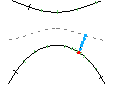
\includegraphics[width=\linewidth]{figs/admissibility_motivation2.pdf}
  \end{minipage}\hfill
  \begin{minipage}{.33\textwidth}
    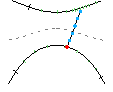
\includegraphics[width=\linewidth]{figs/admissibility_motivation1.pdf}
  \end{minipage}\hfill
  \begin{minipage}{.33\textwidth}
    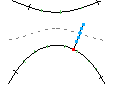
\includegraphics[width=\linewidth]{figs/admissibility_motivation3.pdf}
  \end{minipage}\hfill
  \mcaption{fig:admissibility-motivation}{Possible check point configurations}{A \twod  example depicting three choices of $a$ and $b$ in \cref{eq:check}. 
 Shown is the boundary $\Gammah$, with black tick marks denoting patch boundaries of $\Pcoarse$, green tick marks denoting patch boundaries of $\Pfine$, the target point (red dots), its check points (blue dots) along the normal closest to the target point, and the medial axis of $\Gammah$ (gray dotted line).
Large (left) and small (middle) values of $a$ and $b$ can cause clustering of check points near to $\Gammah$, which requires large amounts of upsampling to compute the potential accurately. Using the medial axis as a heuristic to for admissibility (right), we can minimize the amount of adaptive upsampling required.}
\end{figure}
In \Cref{fig:admissibility-motivation}, we show three examples of different choices of check point locations to evaluate the potential at a point with \qbkix. 
%Suppose that we have chosen extrapolation parameters $a$ and $b$ such that the extrapolation accuracy is less then $\etrg$, following the discussions in \cref{sec:extrap_error,sec:parameter-selection}. From an accuracy perspective, each choice of parameters is are equally valid. 
%However, each choice will require a different set $\Pfine$ in order to ensure accurate integration in \cref{eq:double_layer_disc}.
In \cref{fig:admissibility-motivation}-left, $\vc_0$ is placed close to the target point, while in \cref{fig:admissibility-motivation}-middle, $\vc_0$ is far from the target point, but $\vc_p$ is close to a non-local piece of $\Gammah$. 
Both cases will require excessive refinement of $\Pcoarse$ in order to resolve \cref{eq:double_layer_disc} accurately with $\Pfine$.
On the other hand, in \cref{fig:admissibility-motivation}-right, we can either perform one refinement step on $\Pcoarse$ or adjust $a$ and $b$, which will result in fewer patches in $\Pfine$, and therefore provide a faster integral evaluation, while maintaining accuracy.

In an attempt to strike this balance between speed and accuracy, we need certain constraints on the geometry of $\Gammah$ to ensure the efficient and accurate application of \qbkix, which we impose on the patch sets $\Pcoarse$ and $\Pfine$.
We will first outline our constraints on the quadrature patch sets $\Pcoarse$ and $\Pfine$ which allow for accurate evaluation with \qbkix.

\subsubsection{Admissibility criteria\label{sec:admissible}}
A set of patches $\qP$ is \textit{admissibile} if the following statements are satisfied on each quadrature patch in $\qP$:
\begin{criteria}
  \item The error of a surface patch $\vP_i$ approximating an embedding $\gamma_r$ is below some absolute target accuracy $\err{g}$ \label{criteria:1}
  \item The interpolation error of the boundary condition $f$ is below some absolute target accuracy $\err{f}$ \label{criteria:2}
  \item For each check center $\vhc_j$ corresponding to the quadrature point $\vy_j$ on the surface, the closest point on $\hat{\Gamma}$ to $\vhc_j$ is $\vy_j$. \label{criteria:3}
%  \item Each patch has characteristic length $L \geq L_\lbl{min}$.\label{criteria:4}
\end{criteria}

\Cref{criteria:1} is required to ensure that $\Gammah$ approximates $\Gamma$ with sufficient accuracy to solve the integral equation.
We discuss how to choose $\err{g}$ in \cite[Section 6]{morse2020bsupplementary}; for the tests in this paper, we simply choose $\err{g} < \err{target}$.
\Cref{criteria:2} guarantees that $f$ can be represented at least as accurately as the desired solution accuracy.
We therefore similarly choose $\err{f} < \etrg$. 
%The parameters $a$ and $b$ in \cref{eq:check} are chosen to place check points to balance the extrapolation error, which grows as $a$ and $b$ increase, and smooth quadrature error, which grows as $a$ and $b$ decrease, while attempting to minimize cost.
\Cref{criteria:3}  balances the competing geometric constraints of cost and accuracy by flexibly placing check points as far as possible from $\Gammah$ without causing too much upsampling on other patches.
%Rather than checking all check point locations individually, we use the check center $\vhc$ as a proxy.
If a check point $\vc$ constructed from a surface patch $\vP$ is too close to another surface patch $\vP'$, \Cref{criteria:3} will indicate that $\vP$ is inadmissible. 
If $\vP$ is subdivided into its children, new check points $\vc^\prime$ generated from these children of $\vP$ will be closer to $\vP$ and further from $\vP'$.
Since check points are placed at distances proportional to $L(\vP)$, repeated refinement of $\vP$ will eventually satisfy \Cref{criteria:3}. 

\subsubsection{Upsampling criteria\label{sec:adaptive_upsampling}}
Once we have a set of admissible surface patches satisfying \Cref{criteria:1,criteria:2,criteria:3}, we need to determine the upsampled quadrature patches $\Pfine$ that ensure that the check points generated from $\Pcoarse$ are in $\Omega_I$, i.e., $\|u(\vc) - \hat{u}(\vc, \Pfine)\| < \etrg$.
%Once the set of admissible surface patches $\Pcoarse$ is computed, we need to determine the upsampled quadrature patches $\Pfine$ that ensure that the check points generated from $\Pcoarse$ are in $\Omega_I$, i.e., $\|u(\vc) - \hat{u}(\vc, \Pfine)\| < \etrg$.
To achieve this, we need a criterion to determine which patches are ``too close'' to a given check point for the error to be below $\err{target}$.
We make the following assumption about the accuracy of our smooth quadrature rule: \textit{\cref{eq:double_layer_disc} is accurate to $\err{target}$ at points further than  $L(\vP)$ from $\vP$, for $\err{target} > 10^{-12}$}.
This is motivated by \cite{aT2,barnett2014evaluation}, which demonstrate the rapid convergence of the layer potential quadrature error with respect to $\|\vx - \vsx\|_2$.  
For sufficiently high quadrature orders, such as $q=20$, this assumption seems to hold in practice.
We say that a point $\vx$ is \textit{near} to $\vP$ if the distance from $\vx$ to $\vP$ is less than $L(\vP)$; otherwise, $\vx$ is \textit{far} from $\vP$.
We would like all check points required for the singular/near-singular evaluation of the discretization of \cref{eq:double_layer} using \qbkix to be far from all patches in $\Pfine$.
If this is satisfied, then we know that the Clenshaw-Curtis quadrature rule will be accurate to $10^{-12}$ at each check point.

\subsection{Refinement algorithm preliminaries}
Computing the distance from a check point to a given patch is a fundamental step in verifying the constraints on $\Pcoarse$ and $\Pfine$ from \cref{sec:admissible,sec:adaptive_upsampling}. 
Before detailing our refinement algorithms to enforce these criteria, we introduce several geometric algorithms and data structures that will be used to compute the closest point on piecewise polynomial surfaces.

\subsubsection{\aabb trees\label{sec:aabb_trees}} 
In order to implement our algorithms to enforce admissibility efficiently, we use a fast spatial data structure to find the patches that are close to a query point $\vx$.
In \cite{RKO, wala20193d}, the quadtree and octree within an \fmm is extended to support the geometric queries needed for a fast \qbx  algorithm.
In this work, we use an axis-aligned bounding box (\aabb) tree, which is a type of bounding volume hierarchy \cite{samet2006foundations}, implemented in \texttt{geogram} \cite{geogram}.
An \aabb is a tree with nodes corresponding to bounding boxes and leaves corresponding to bounding boxes containing single objects. 
A bounding box $B_0$ is a child of another box $B_1$ if $B_0 \subset B_1$; the root node is a bounding box of the entire domain of interest.
Operations supported by \aabb trees include: (i) finding all bounding boxes containing a query point, (ii) finding all bounding boxes that intersect another query box, (iii) finding the closest triangle to a query point (because triangles have trivial bounding boxes). 
By decoupling geometric queries from fast summation, the individual algorithms can be more thoroughly optimized, in exchange for the additional memory overhead of maintaining two distinct data structures.
The query algorithm presented in \cite{lu2019scalable} likely has better parallel scalability, but \aabb trees are faster for small to medium problem sizes on a single machine due to less redundant computation.

To define an \aabb tree for our patch-based surface $\Gammah$, we make use of the following fact: the control points of a B\'ezier surface ($\vector{a}_{\ell m}$'s from \cref{eq:tensor-product}) form a convex hull around the surface that they define \cite{F}.
As a result, we can compute a bounding box of a surface or quadrature patch $\vP$ directly from the B\'ezier coefficients simply by computing the maximum and minimum values of each component of the $\vector{a}_{\ell m}$'s, as shown in \cref{fig:patch-coeffs-bbox}-middle.
This bounding box can then be inserted into the \aabb tree as a proxy for a surface or quadrature patch.
\begin{figure}[!htb]
  \centering
  %\setlength\figureheight{1.9in}
  %\setlength\figurewidth{2.1in}
  \begin{minipage}{.33\textwidth}
      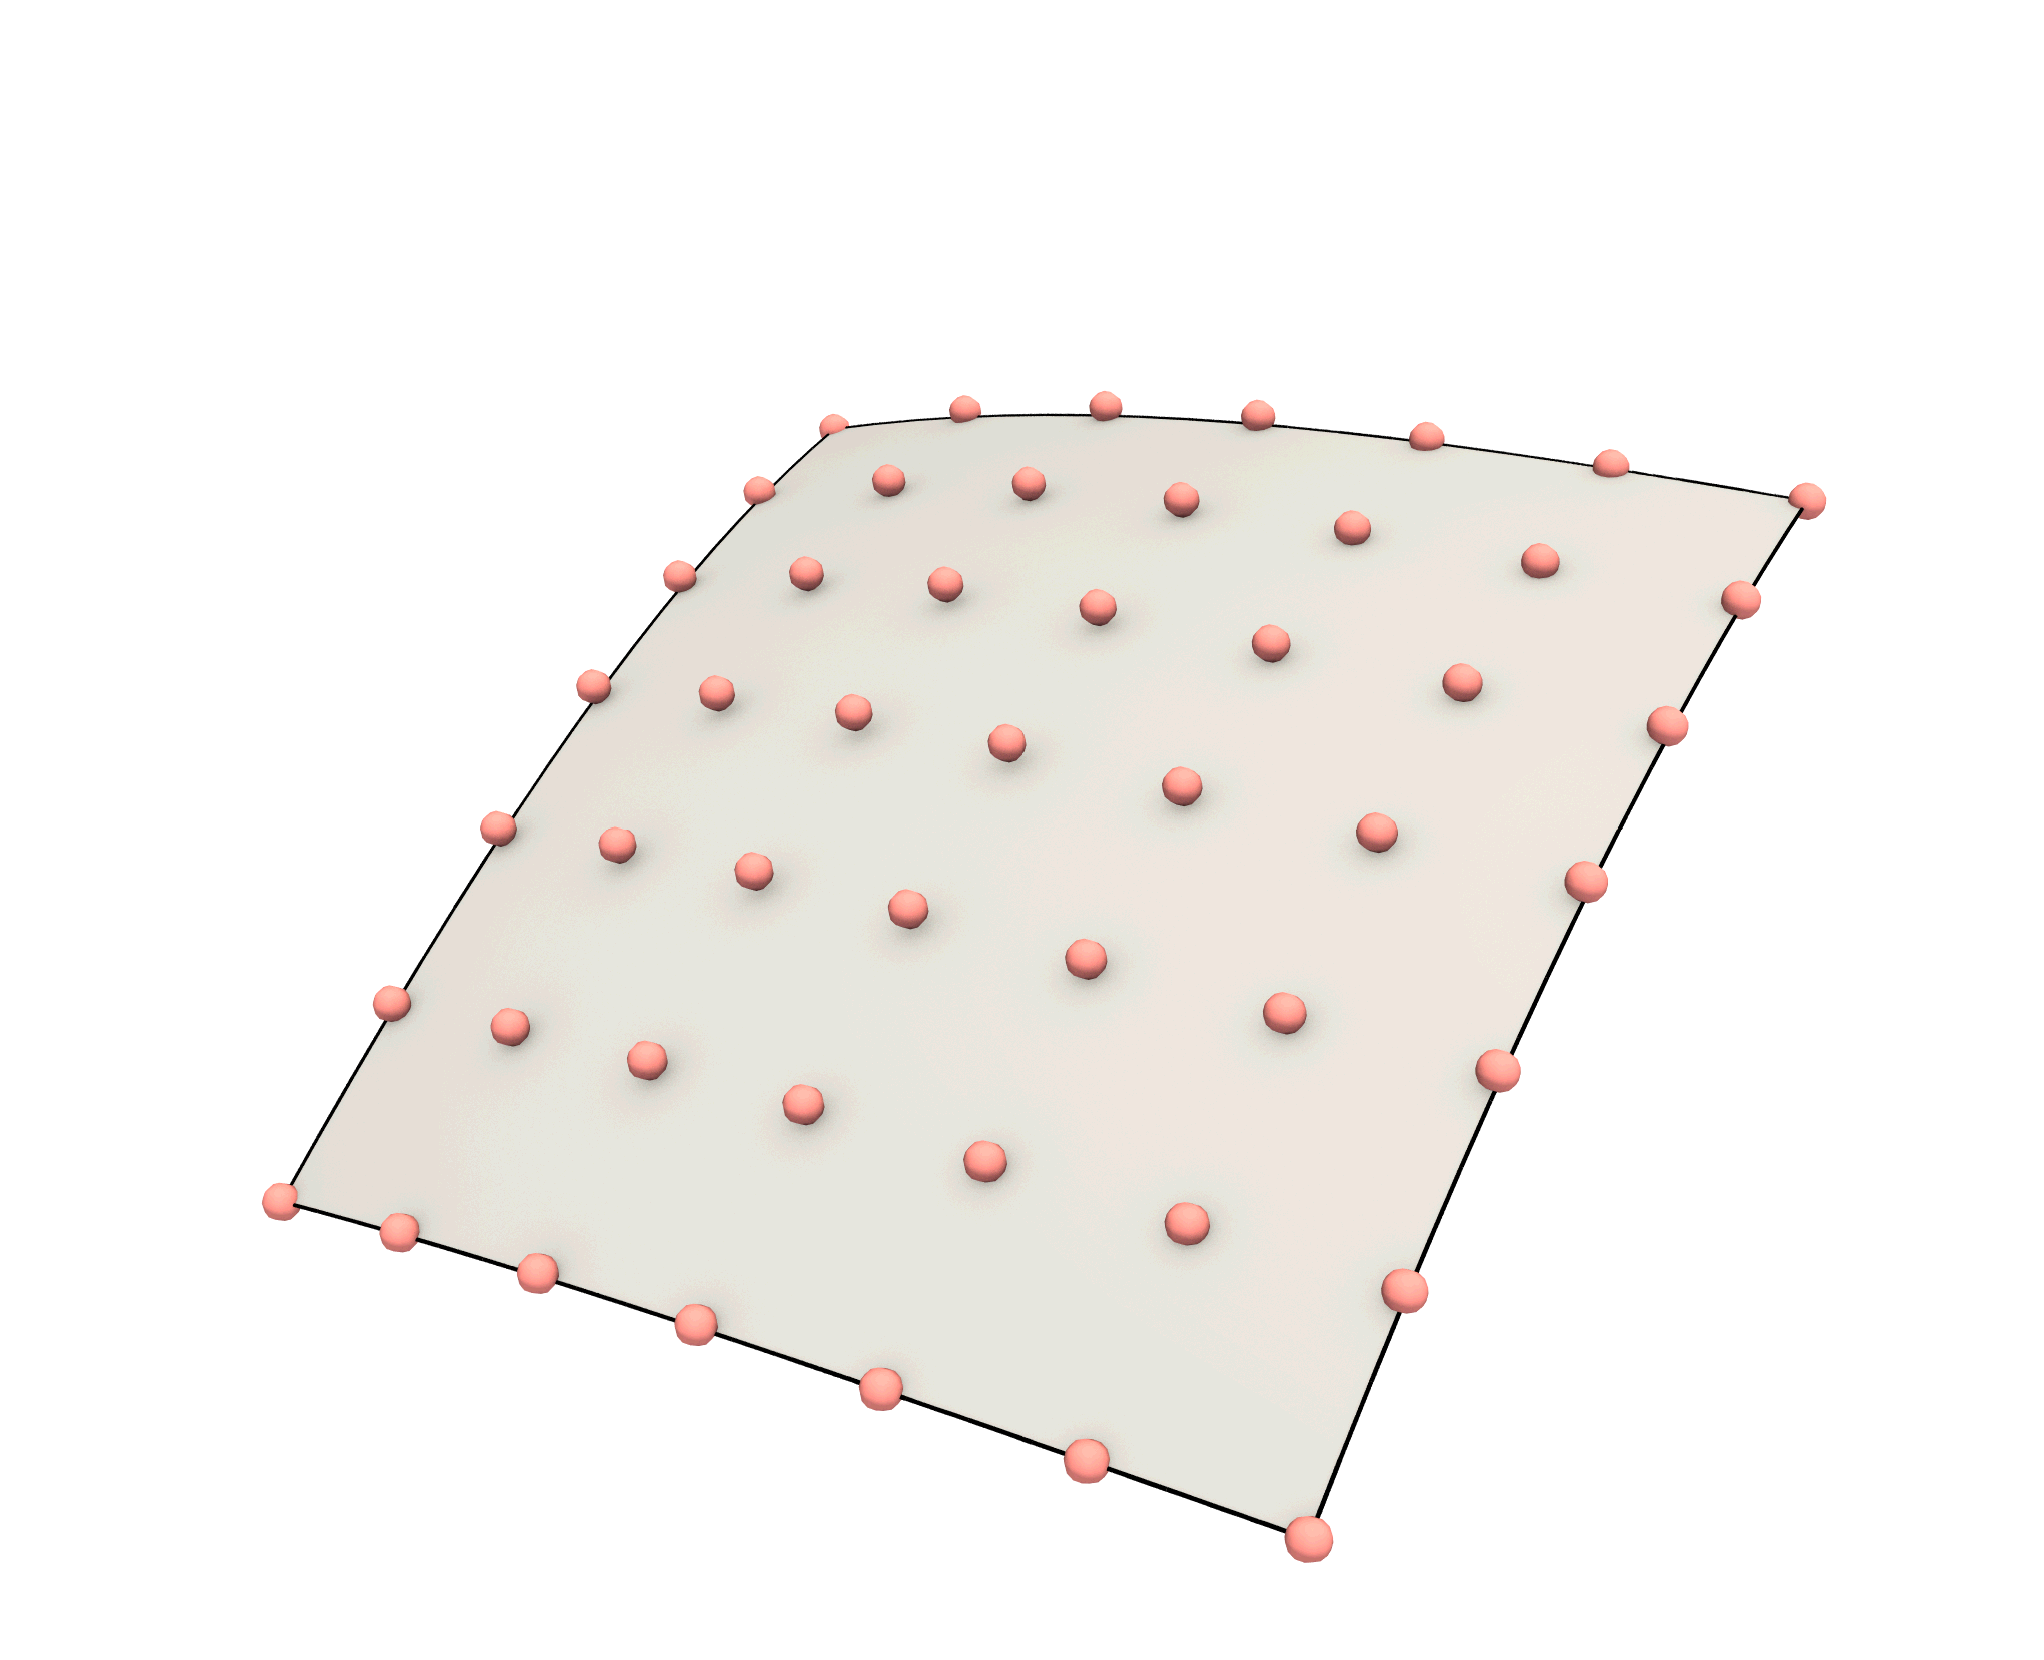
\includegraphics[width=\linewidth]{figs/patch_with_coeffs.png}
  \end{minipage}\hfill
  \begin{minipage}{.33\textwidth}
    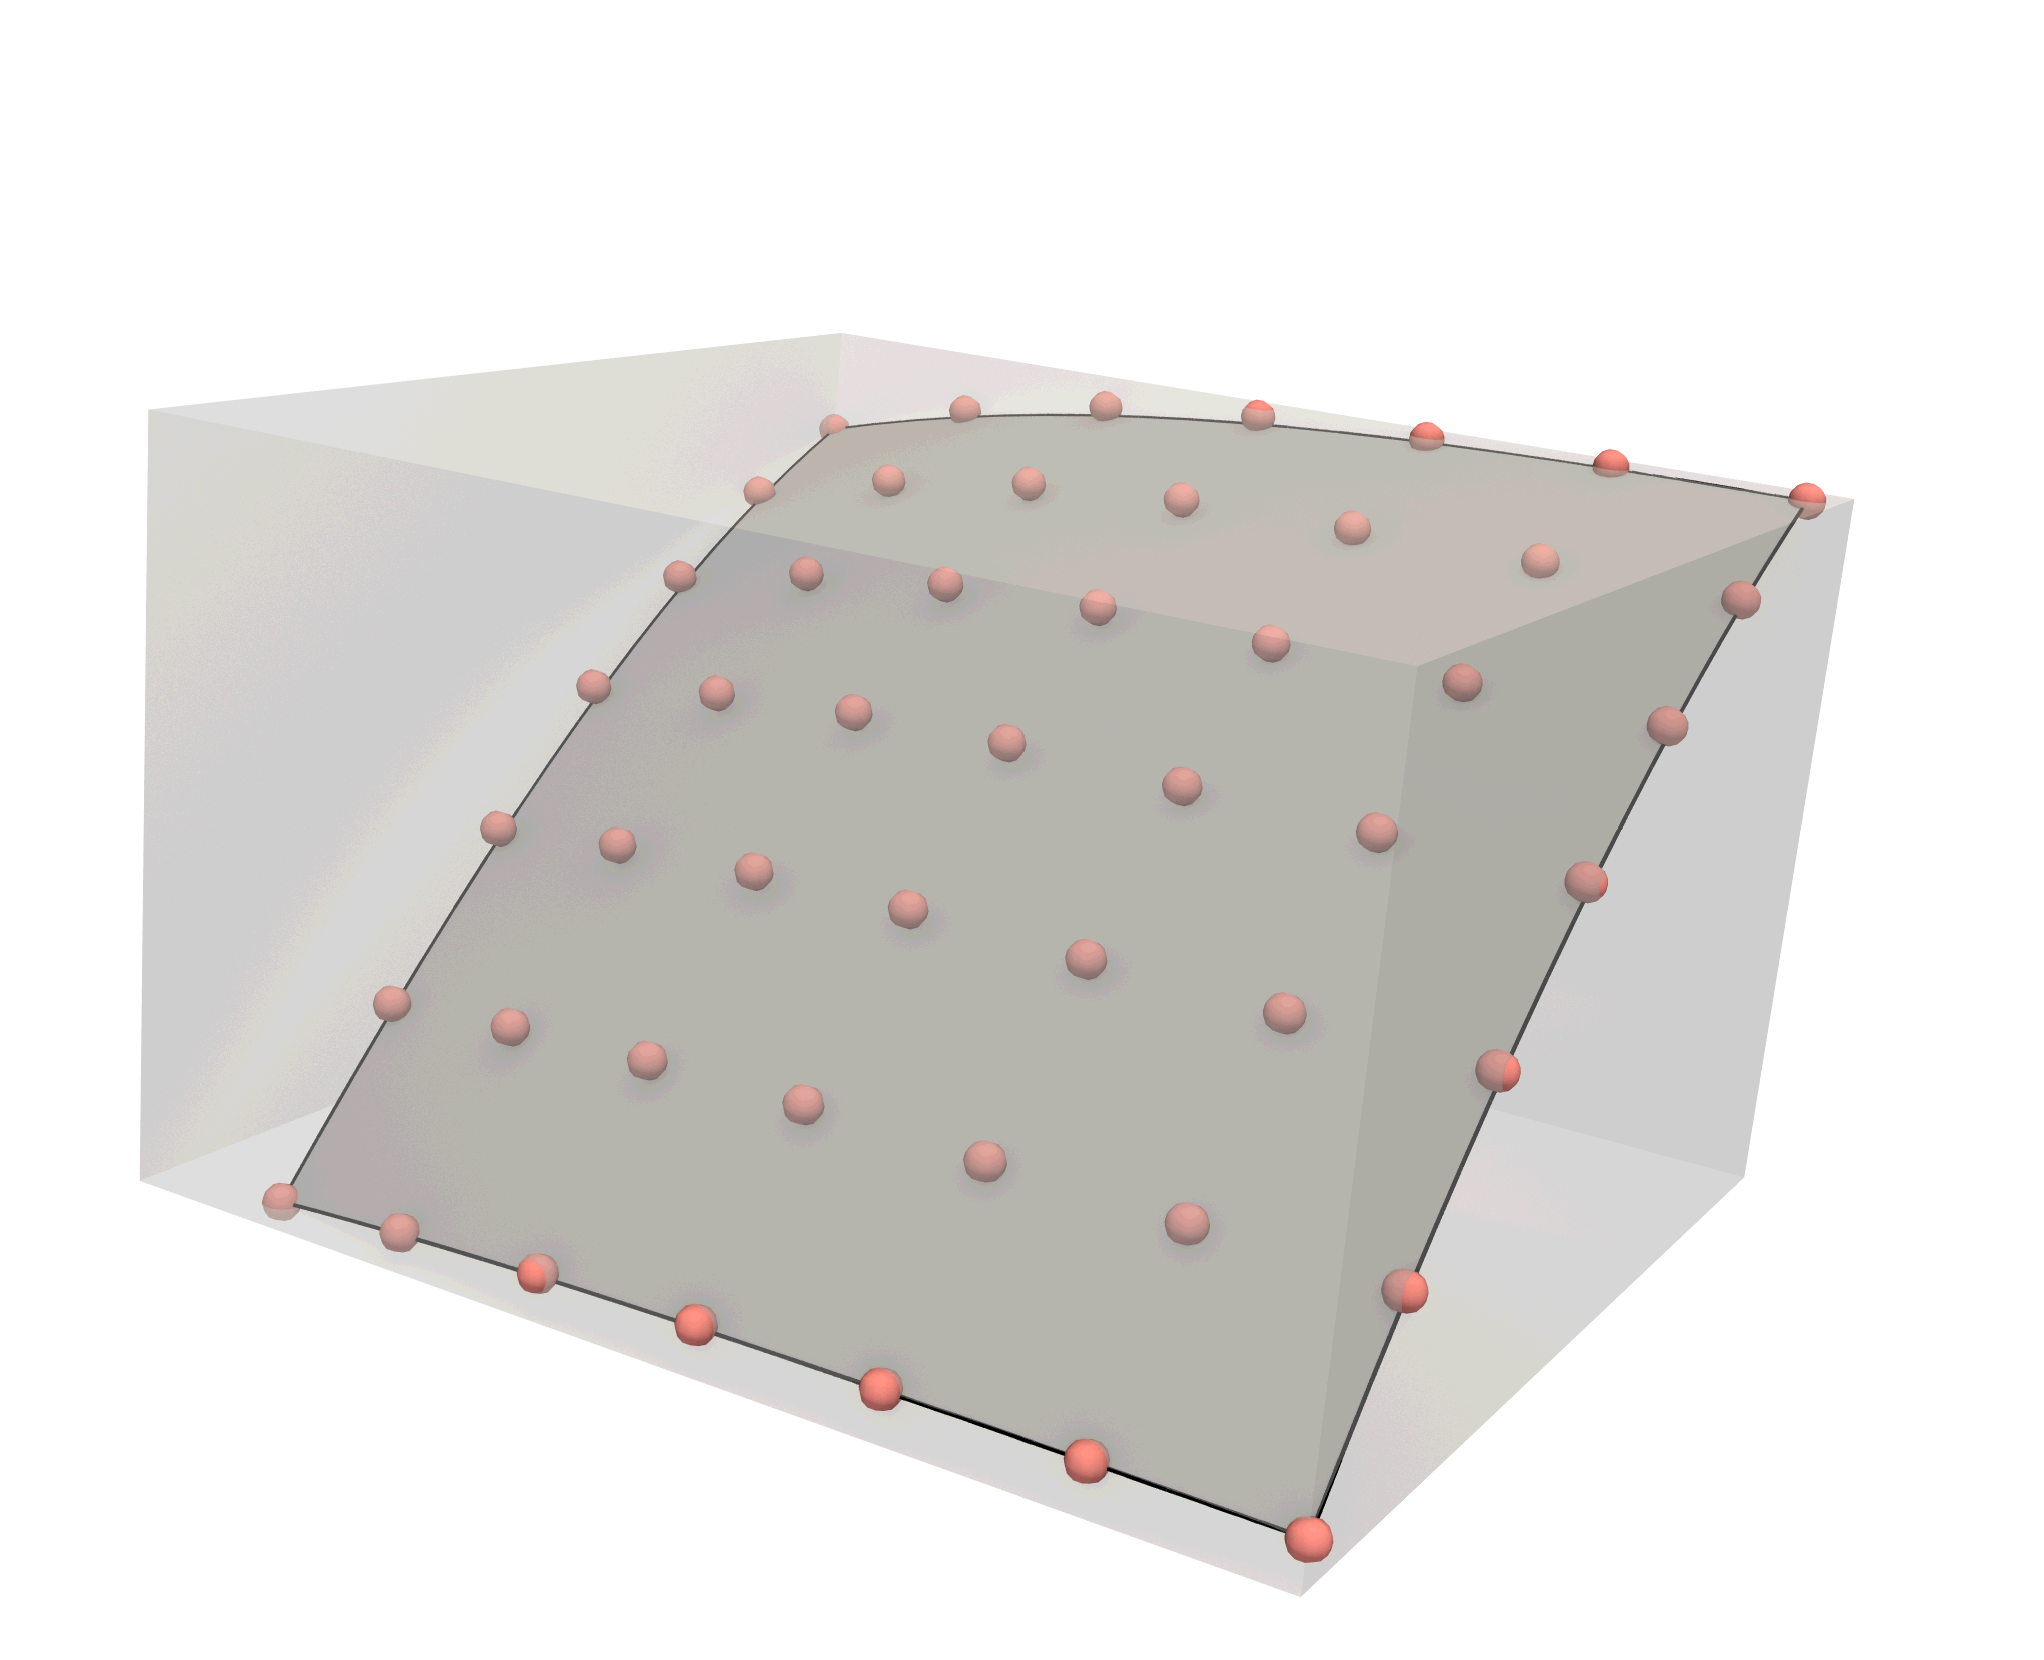
\includegraphics[width=\linewidth]{figs/patch_with_coeffs_bbox.png}
  \end{minipage}\hfill
  \begin{minipage}{.33\textwidth}
    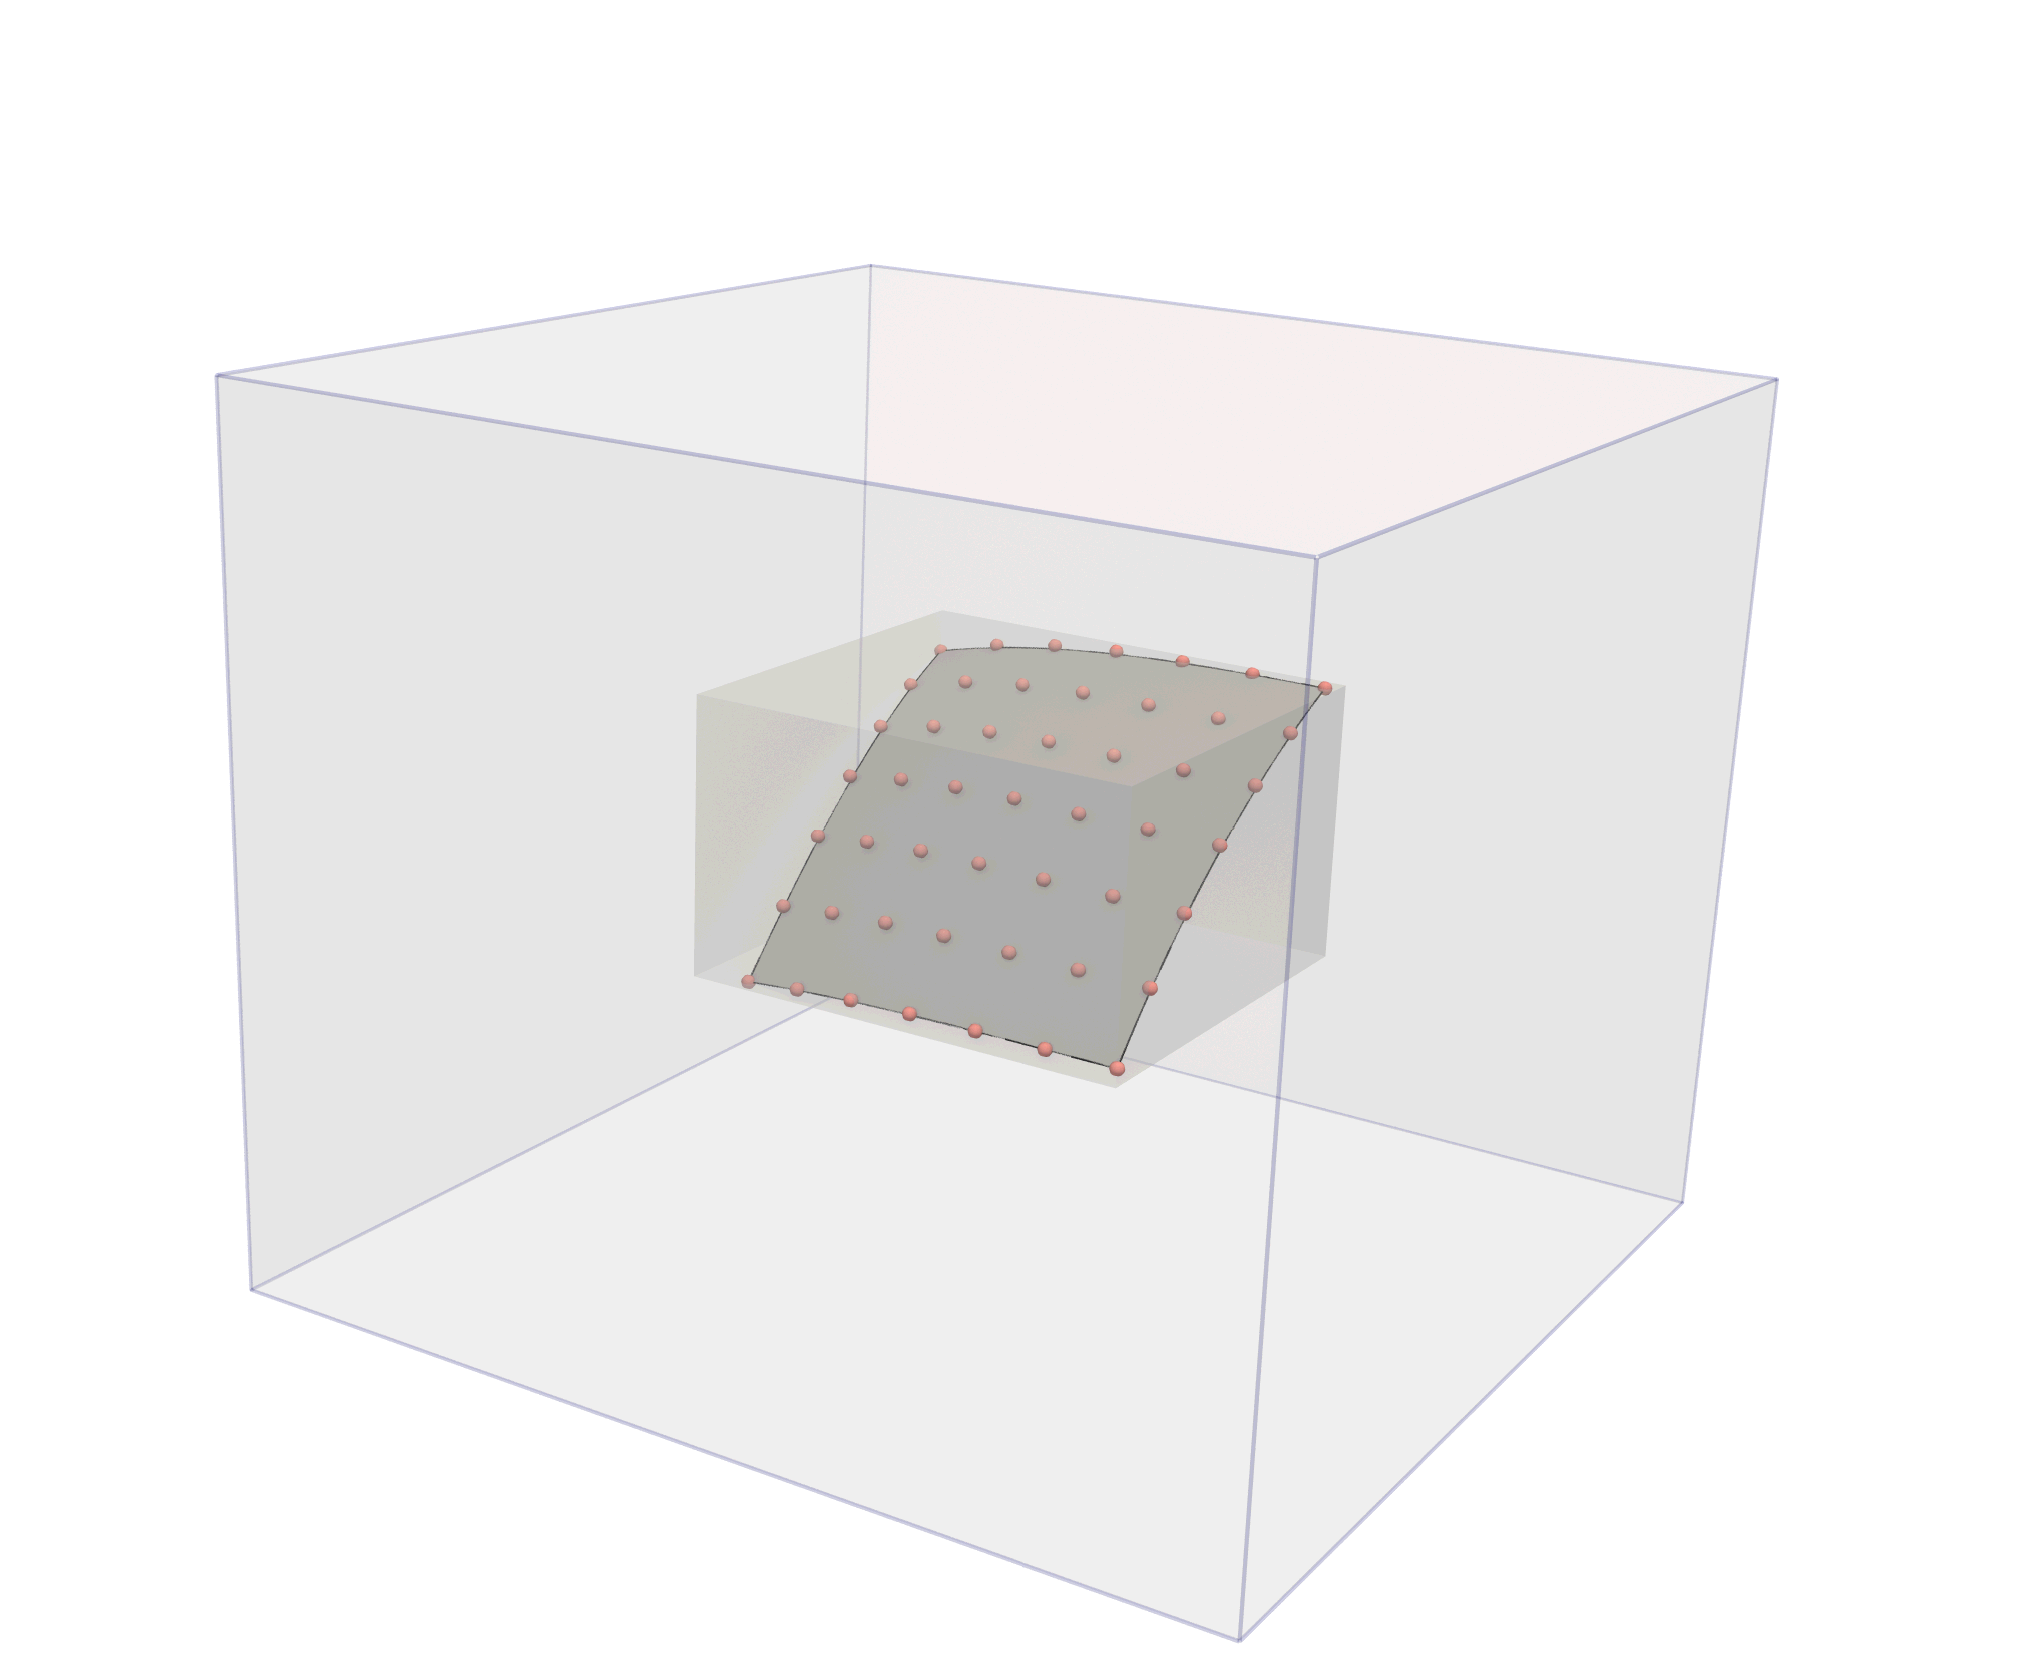
\includegraphics[width=\linewidth]{figs/patch_with_coeffs_near_bbox.png}
  \end{minipage}\hfill
  \mcaption{fig:patch-coeffs-bbox}{Relationship between control points and
  bounding boxes}{Left: a patch in the tensor product B\'ezier basis, with control
      points ($\vector{a}_{\ell m}$'s from \cref{eq:tensor-product}) plotted. The convex hull of the control points of a patch are guaranteed
      to contain the patch. Center: The patch bounding box, computed from the control
      points. Right: The near-zone bounding box of the patch from
      \cref{sec:adaptive_upsampling_algo} computed by
      inflating the bounding box by $L(\vP)$.
}
\end{figure}



\subsubsection{Computing the closest point to a patch\label{sec:closest_point_algo}}

To find a candidate closest patch $\vP_{i_0}$ to $\vx$, we construct a fine triangle mesh and bounding boxes of each patch in $\Pcoarse$ and insert them into an \aabb tree.
We can query the \aabb tree for the nearest triangle to $\vx$ with the \aabb tree, which corresponds to $\vP_{i_0}$.
We then compute the accurate true distance $d_{i_0}$ to $\vP_{i_0}$ using a constrained Newton method, presented in detail in \cite[Section 2]{morse2020bsupplementary}.

However, there may be other patches whose distance to $\vx$ is less than $d_{i_0}$, as shown in \cref{fig:candidate-near-patch}.
To handle this case, we then query the \aabb tree for all patches $\vP_{i_1}, \hdots, \vP_{i_k}$ that are distance at most $d_{i_0}$ from $\vx$.
This is achieved by forming a query box centered at $\vx$ with edge length $2d_{i_0}$ and querying the \aabb tree for all intersection bounding boxes. 
The precise distance is then computed for each patch  $\vP_{i_1}, \hdots, \vP_{i_k}$ with \cite[Section 2]{morse2020bsupplementary} and the smallest distance is chosen.
We summarize this process in \cref{alg:closest_point}.


\begin{algorithm}[!htp]
    \KwData{A set of quadrature patches $\qP$, a query point $\vx$, Newton method tolerance $\err{opt}$}
  \KwResult{The closest point $\vsx$ on $\qP$ to $\vx$}

  \DontPrintSemicolon
  Construct an AABB tree $T_T$ from a fine triangle mesh of the quadrature patches of $\qP$\;
  Construct an AABB tree $T_B$ from bounding boxes of quadrature patches in $\qP$.\;
    $\tau_0 = $ closest triangle to $\vx$ computed with $T_T$ \;
  
    $\vP_{i_0} = $ patch corresponding to $\tau_0$\;
    Find the closest point $\vector{s}_{\vector{\vx},0}$ on $\vP_{i_0}$ to $\vx$ with \cite[Section 2]{morse2020bsupplementary}.\;
    $d_{i_0} = \|\vx - \vector{s}_{\vector{\vx},0}\|_2$\;
    $B_{d_{i_0}}(\vx)=$ a box centered a $\vx$ with edge length $2d_{i_0}$\;
    Find the boxes $B_{i_1}, \hdots B_{i_k}$ in $T_B$ that intersect $B_{d_{i_0}}(\vx)$\;
    
    \For{$B_{i_j} \in B_{i_1}, \hdots B_{i_k}$}{
      $\vP_{i_j} =$ quadrature patch corresponding to $B_{i_j}$ \;
      Find the closest point $\vector{s}_{\vector{\vx},j}$ on $\vP_{i_j}$ to $\vx$ with \cite[Section 2]{morse2020bsupplementary} to precision $\err{opt}$.\;
      $d_{i_j} = \|\vx - \vector{s}_{\vector{\vx},j}\|_2$\;
    }
    $j^* = \mathrm{argmin}_j\{d_{i_j}\}$ \;
    \Return{$\vector{s}_{\vector{x},j^*}$}
  \mcaption{alg:closest_point}{Compute the closest point to $\vx$}{}
\end{algorithm}

\begin{figure}[!htb]
  \centering
  %\setlength\figureheight{1.9in}
  %\setlength\figurewidth{2.1in}
  \hfill
  \begin{minipage}{.3\textwidth}
      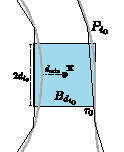
\includegraphics[width=\linewidth]{figs/candidate_near_patch_trimesh.pdf}
  \end{minipage}\hfill
  \mcaption{fig:candidate-near-patch}{A \twod schematic of near-patch candidate selection}{
      A visual depiction of the quantities defined in lines 3-7 of \cref{alg:closest_point} (shown here in \twod for simplicity), with notation matching \cref{alg:point_marking}.
      The triangle-mesh proxy is drawn in as black lines and patches are drawn as gray curves.
      We have found an initial closest triangle $\tau_0$ to $\vx$ corresponding to patch $\vP_{i_0}$ and computed $d(\vx, \vP_{i_0}) = d_{i_0}$.
      We then query the \aabb tree for all patches that intersect box $B_{d_{i_0}}$ with edge length $2d_{i_0}$, shown in blue.
      There is clearly a patch that is closer to $\vx$ than $\vP_{i_0}$ that will be returned from the query, which will be distance $d_\lbl{min}$ from $\vx$.
}
\end{figure}

\subsection{Admissibility algorithm\label{sec:admissible_algo}}
Our algorithm to enforce \cref{criteria:1,criteria:2,criteria:3} proceeds as follows:
\begin{itemize}
    \item To enforce \Cref{criteria:1}, we adaptively fit a set of surface patches to the embeddings $\gamma_r$ representing $\Gamma$.
We construct a bidegree $(n,n)$ piecewise polynomial least-squares approximation $\vP_i$ in the form of \cref{eq:tensor-product} to $\gamma_r$ on $I^2$.
        If $\vP_i$'s domain $\mathcal{D}_i$ is obtained by refinement of $E_r$, we fit $\vP_i \circ \eta_i$ to $\gamma_r$ on $\I^2$, using $4n \times 4n$ samples on $\I^2$. 
        If the pointwise error of $\vP_i$ and its partial derivatives is greater than $\err{g}$, then it is quadrisected and the process is repeated. 

\item  Once the embeddings are resolved, we resolve $f$ on each surface patch produced from the previous step in a similar fashion to enforce \Cref{criteria:2}.
  However, rather than a least-squares approximation in this stage, we use piecewise polynomial interpolation.
 
\item To enforce \Cref{criteria:3}, we construct the set of check centers $\vhc_I$ which correspond to the check points required to evaluate the solution at the quadrature nodes $\vy_I$.
    For each check center $\vhc_I$, we find the closest point $\vector{s}_{\vhc_I} \in \Gammah$.
    If $ \|\vector{s}_{\vhc_I} - \vy_I\| \geq \err{opt}$, we split the quadrature patch $\vP$ containing $\vy_I$.
        The tolerance $\err{opt}$ is used in the Newton's method in \cite[Section 2]{morse2020bsupplementary}; we usually choose $\err{opt}=10^{-14}$.
Since $d(\vhc_I,\Gammah)$ is proportional to $L_{\vy_I}$, the new centers $\vhc_I$ for the refined patches  will be closer to the surface. 
    We use \cref{alg:closest_point} to compute $\vector{s}_{\vhc_I}$.
        However, in the case of check points, we can skip lines 1-6 to compute $d_{i_0}$,  since $\vhc_I$ is $R + r(p+1)/2$ away from $\vy_I \in \vP(D)$ by construction.
        We can apply lines 7-14 of \cref{alg:closest_point} with $d_{i_0} = R + r(p+1)/2$ to compute $\vector{s}_{\vhc_I}$.
\end{itemize}

We summarize the algorithm to enforce \Cref{criteria:3} in \cref{alg:admissibility}.
At each refinement iteration, the offending patches are decreased by quadrisection, which reduces the distance from the quadrature point $\vy_I$ to its checkpoints.
This eventually satisfies \Cref{criteria:3} and the algorithm terminates. 

\begin{algorithm}[!ht]
  \KwData{A set of quadrature patches $\qP$, optimization tolerance $\err{opt}$}
  \KwResult{An admissible set of quadrature patches $\qP$}

  \DontPrintSemicolon
  $\qP = \Pcoarse$\;
  Mark all patches in $\qP$ as inadmissible.\;
  
  \While{any patch in $\qP$ is inadmissible}{
    Construct an AABB tree $T$ as described in \cref{sec:closest_point_algo} from $\qP$\;
    \For{$\vP \in \qP$}{
        \If{$\vP$ is inadmissible}{
            Construct a set of check centers $C_\vP$ for each $\vy_J \in \vP(D)$ \;

            \For{$\vhc \in C_\vP$}{
                $d_{i_0} = R + r(p+1)/2$\;
                Compute $\vector{s}_\vhc$ with lines 7-14 of \cref{alg:closest_point} with precision $\err{opt}$ and $d_{i_0}$.\;
                %Construct a box $B(\vhc)$ with edge length $2R + r(p+1)$ centered at $\vhc$.\;
                %$B_{i_1}, \hdots B_{i_k}$ = \texttt{query\_bbox\_intersections}($T$, $B(\vhc)$\texttt)\;
                %$P_{i_1}, \hdots P_{i_k}$ =  patches corresponding to $B_{i_1}, \hdots B_{i_k}$\;
                %\eIf{$P \in \{P_{i_1}, \hdots P_{i_k}\}$}{
                %    Compute candidate closest points $\vector{s}_\vhc^{(1)}, \hdots \vector{s}_\vhc^{(k)}$ on $P_{i_1}, \hdots P_{i_k}$ to $\vhc$ with \cref{app:closest_point} to accuracy $\err{opt}.$\;
                %    $\vector{s}_\vhc = \mathrm{argmin}_i \|\vector{s}_\vhc^{(i)}, - \vhc\|_2$\;
                \eIf{$\|\vector{s}_\vhc -\vy_J\|_2 < \err{opt}$}{
                    Mark $\vP$ as admissible.\;
                } {
                    Mark $\vP$ as inadmissible.\;
                    break   \tcp{only need one bad check center to mark $\vP$ for refinement}
                }
            }
        }
    }
    \For{$\vP \in \qP$}{
      \If{$\vP$ is inadmissible}{
        Split $\vP$ into its four child patches, mark each as inadmissible, and replace $\vP$ with its children in $\qP$.
      }
    }
  }
  \Return{$\qP$}
  \mcaption{alg:admissibility}{Enforce admissibility \Cref{criteria:3} on a set of quadrature patches}{}
\end{algorithm}

\subsection{Adaptive upsampling algorithm \label{sec:adaptive_upsampling_algo}}
%Simply applying the point marking algorithm detailed \cref{app:point_marking} to each check point is not sufficient.
Before detailing our upsampling algorithm to satisfy the criteria outlined in \cref{sec:adaptive_upsampling}, we must define the notion of a \textit{near-zone bounding box} of a quadrature patch $\vP$, denoted $B_\lbl{near}(\vP)$.
The near-zone bounding box of $\vP$ is computed as described in \cref{sec:aabb_trees}, but then is inflated by $2L(\vP)$, as shown in \cref{fig:patch-coeffs-bbox}-right.
This inflation guarantees that any point $\vx$ that is near $\vP$ is contained in $B_\lbl{near}(\vP)$ and, for an admissible set of quadrature patches $\Pcoarse$, that any $\vx\in \Omega_N$ must be contained in some quadrature patch's near-zone bounding box.
This means that by forming $B_\lbl{near}(\vP)$ for each quadrature patch in $\Pfine$, a check point is in $\Omega_I$ if it is not contained in any near-zone bounding boxes.

To compute the upsampled patch set from $\Pcoarse$, we initially set $\Pfine = \Pcoarse$, compute the near-zone bounding boxes of each patch in $\Pfine$ and insert them into an \aabb tree.
We also construct the set of check points $C$ required to evaluate our discretized layer-potential with \qbkix (\cref{sec:singular-eval}).
For each check point $\vc \in C$, we query the \aabb tree for all near-zone bounding boxes that contain $\vc$.
If there are no such boxes, we know $\vc$ is far from all quadrature patches and can continue.
If, however, there are near-zone bounding boxes $B_{i_0},\hdots, B_{i_k}$ containing $\vc$, we compute the distances $d_{i_k}$ from $\vc$ to $\vP_{i_1},\hdots,\vP_{i_k}$ using \cite[Section 2]{morse2020bsupplementary}.
If $d_{i_k} < L(\vP_{i_k})$, we replace $\vP_{i_k}$ in $\Pfine$ with its four children produced by quadrisection.


To improve the performance of this refinement procedure, we allow for the option to skip the Newton method in \cref{alg:closest_point} and immediately refine all patches $\vP_{i_0},\hdots \vP_{i_k}$.
This is advantageous in the early iterations of the algorithm, when most check points are near to patches by design.
We allow for a parameter $n_\lbl{skip}$ to indicate the number of iterations to skip the Newton optimization and trigger refinement immediately.
We typically set $n_\lbl{skip}=2$.
We summarize our algorithm in \cref{alg:adaptive_upsampling}.
%We first use the error estimate of \cref{sec:quad_error_heuristic} to determine the distance from the intermediate field $\Omega_I$ to the patch $P$,  which we will call $d_\lbl{near}(P)$.
%We compute a bounding box of $P$ as described in \cref{sec:mark_near}.
%We compute a bounding box of each patch $P$ in $\Pfine$ as described in \cref{sec:aabb_trees}.
%We then inflate the box size by $2d_\lbl{near}$ to produce the \textit{near-zone bounding box} of $P$, denoted $B_\lbl{near}(P)$, as shown in \cref{fig:patch-coeffs-bbox}-right. 
%We then inflate the each boxes' size by $2L(P)$ to produce the \textit{near-zone bounding box} of $P$, denoted $B_\lbl{near}(P)$, as shown in \cref{fig:patch-coeffs-bbox}-right. 

%However, we need to still determine if a point $\vc$ in $B_\lbl{near}(P)$ is actually near to $P$, which requires computing the distance from $\vc$ to $\Gammah$.

%To check this efficiently, we insert all the near-zone bounding boxes into an \aabb tree. 
%Let $C$ be the set of all check points required to evaluate our discretized layer potential.
%For each check point $\vc \in C$, we query the tree for all boxes containing $\vc$.
%The set of quadrature patches corresponding to the returned set of boxes are candidate patches for upsampling.
%We can now check the distance from $\vc$ to each of these quadrature patches using \cref{app:closest_point} and trigger refinement if the distance between $\vc$ and a given patch is less than $L$.
%Alternatively, one can also simply trigger refinement on all of the patches returned by the \aabb tree query without explicitly checking the distance.
%This is a cheaper operation that avoids the Newton iterations of \cref{app:closest_point}, but is less accurate and can cause over-refinement.
%One can either trigger upsampling on all of these patches or explicitly compute the distance from $\vc$ to each quadrature patch using .
%The former is a cheaper condition to check but less accurate; the latter is more precise and triggers less upsampling overall, but more expensive.
%This bounding box proxy is an over-approximation of $\Omega_N$; there are many cases in which a check point is contained in a near-zone bounding box, but strictly in $\Omega_I$.
%In these cases, the true distance from $\vc$ to each quadrature patch is more accurate.
%We strike a balance by triggering upsampling for all returned quadrature patches for the first iteration or two of upsampling and explicitly check distance to patches for the remaining iterations.

%The set $C$ is determined by $\Pcoarse$ and therefore fixed. 
%The average size of near-zone bounding boxes decreases after each step of refinement until the algorithm terminates; eventually no near-zone bounding boxes will contain check points.
%We summarize in \cref{alg:adaptive_upsampling}.

\begin{algorithm}[!htp]
    \KwData{An admissible patch set $\qP$, number of iterations $n_\lbl{skip}$ before using \cite[Section 2]{morse2020bsupplementary}}
  \KwResult{An upsampled set of quadrature patches}
  
  \DontPrintSemicolon
  Compute inflated near-zone bounding boxes $B_1, \hdots,  B_N$ of each $\vP \in \qP$.\;
  Construct an AABB tree $T$ from the near-zone bounding boxes.\;
  Construct all check points $C$ required to evaluate the \cref{eq:int-eq} on $\qP$.\;

  $\qP_\lbl{fine} = \qP$\;
  Mark all check points in $C$ as near.\;
  $i=0$

  \While{any $\vc \in C$ is marked near}{
    \For{$\vc \in C$}{
        \If{$\vc$ is marked near}{
            Query $T$ for all bounding boxes $B_{i_1}, \hdots B_{i_k}$ containing $\vc$.\;
            $\vP_{i_1}, \hdots \vP_{i_k} = $ patches corresponding to boxes $B_{i_1}, \hdots B_{i_k}$\;
            Mark $\vc$ as far\;
            \For{$\vP \in \vP_{i_1}, \hdots \vP_{i_k}$}{
                \eIf{$i > n_\lbl{skip}$}{
                    Find the closest point $\vector{s}_{\vc}$ on $\vP$ to $\vc$ with \cref{alg:closest_point}.\;
                    %\If{The error estimate in \cref{sec:quad_error_heuristic} is greater than $\eps$ with $d = \|\vy - \vc\|_2$}{
                    \If{ $\|\vector{s}_{\vc} - \vc\|_2 < L(\vP)$}{
                        Split $\vP$ and replace it in $\qP_\lbl{fine}$ with its children. \;
                        Mark $\vc$ as near\;
                    }
                } {
                    Split $\vP$ and replace it in $\qP_\lbl{fine}$ with its children.\;
                    Mark $\vc$ as near\;
                }
 
            }
       }
    }
    $i=i+1$\;

  }
    \mcaption{alg:adaptive_upsampling}{Adaptively upsample to accurately evaluate \cref{eq:double_layer_disc} at check points}{}
\end{algorithm}

%In \cite{RKO}, the panel size of the quadrature rule was tied to the distance of the \qbx expansion center from the boundary.
%This design choice produces an artificial dependence of the quadrature and expansion error, since the global upsampling factor for the fine discretization is determined by the closest expansion to the boundary.
%\cite{wala20193d} first presented an approach that decouples the coarse and fine discretizations; we follow a similar approach here.
%However, their approach does not explicitly depend on surface curvature, which has a dramatic impact on quadrature accuracy, which can lead to unnecessary upsampling.
%By taking advantage of the error heuristic in \cref{sec:error}, we are able to accurately determine quadrature accuracy at a given check point.

\subsection{Marking target points for evaluation\label{app:point_marking}}

Once we have solved \cref{eq:linear_system} for $\phi$ on $\Gammah$, we need the ability to evaluate \cref{eq:double_layer} at an arbitrary set of points in the domain.
For a target point $\vx$, in order apply the algorithm in \cref{sec:singular-eval}, we need to determine whether or not $\vx \in \Omega$ and, if so, whether $\vx $ is in $\Omega_N, \Omega_I$ or $\Omega_F$.
Both of these questions can be answered by computing the closest point $\vsx$ on $\Gammah$ to $\vx$. % with \cref{app:closest_point_opt}.
If $\vn(\vsx)\cdot(\vx - \vsx) < 0$, then $\vx \in \Omega$. 
As we have seen in \cref{sec:adaptive_upsampling}, the distance $\|\vx - \vsx\|$ determines whether $\vx \in \Omega_N,\Omega_I$ or $\Omega_F$.
However, for large numbers of target points, a brute force calculation of closest points on $\Gammah$ to all target points is prohibitively expensive.
We present an accelerated algorithm combining \cref{alg:closest_point} and an \fmm evaluation to require only constant work per target point. 


\subsubsection{Marking and culling far points \label{sec:mark_far}}
A severe shortcoming of \cref{alg:closest_point} is that its performance deteriorates as the distance from $\vx$ to $\Gammah$ increases. 
Consider the case where $\Gammah$ is a sphere with radius $r$ with $\vx$ at its center.
The first stage of \cref{alg:closest_point} returns a single quadrature patch that is distance $r$ from $\vx$; the next stage will return all quadrature patches.
This will take $O(N)$ time to check the distance to each patch.
Even on more typical geometries, we observe poor performance of \cref{alg:closest_point} when $\vx$ is far from $\Gammah$.

%It's important that we can mark points in $\Omega_F$ and mark points as inside or outside $\Omega$ without using \cref{sec:mark_near}.
To address this, we use an additional \fmm-based acceleration step to mark most points far from $\Gammah$ before using applying \cref{alg:closest_point}. 
Our approach is based on computing the generalized winding number \cite{jacobson2013robust} of $\Gammah$ at the evaluation points. 
For closed curves in $\mathbb{R}^2$, the \textit{winding number} at a point counts the number of times the curve travels around that point. 
The \textit{generalized winding number} of a surface $\Gammah$ at a point $\vx \in \mathbb{R}^3$ can be written as 
%\begin{equation}
%\omega_{\Gammah}(\vx) = %\frac{1}{4\pi} W_S(\vx) =
%  \frac{1}{4\pi}\iint_{\Gammah} sin(\phi)d\phi d\theta, \quad (\text{when }\vx =0).
%  \label{eq:gen_winding}
%\end{equation}
%%where $W(\vx)$ is the solid angle subtended by $S$. 
%%This is the projection of $S$ onto the unit sphere centered at $\vx$.
%The integrand can be interpreted as the signed differential solid angle subtended by an infinitesimal surface patch centered at $\vx$.
%
%In our case, $\Gammah$ is composed of a collection of surface patches with independent parametrizations, and can be computed patch by patch.
%%It's clear that the solid angle of $\Gammah$ with respect to $\vx$ is the sum of the solid angles of the surface patches:
%\begin{equation}
%  \omega_{\Gammah}(\vx) = \frac{1}{4\pi}\sum_i \iint_{\gamma_i} sin(\phi)d\phi d\theta.
%  \label{eq:gen_winding_patch}
%\end{equation}
%By a change of variables to Cartesian coordinates, we can rewrite \cref{eq:gen_winding} as 


\begin{equation}
  \omega_{\Gammah}(\vx) = -\frac{1}{4\pi}\int_{\Gammah} \frac{(\vx - \vy) \cdot \vn}{\|\vx - \vy\|^3} d\vy_{\Gammah}
  \label{eq:gen_winding2}
\end{equation}
We recognize this integral as the double-layer potential in \cref{eq:double_layer} for a Laplace problem with $\phi = 1$. 
Its values in $\mathbb{R}^3$ are  \cite{K}:
\begin{equation}
  \omega_{\Gammah}(x) =
  \begin{cases}
    1 & \vx \in \Omega \setminus \Gammah\\
    1/2 & \vx \in \Gammah\\
    0 &  \vx \in \mathbb{R}^3 \setminus \overline{\Omega}
  \end{cases}
  \label{eq:const-density}
\end{equation}
\cref{eq:gen_winding2} can be evaluated using the same surface quadrature in \cref{eq:double_layer_disc} using an \fmm in $O(N)$ time.
While the quadrature rule is inaccurate close to the surface, $\Omega_F$ is defined precisely as the zone where the quadrature rule is sufficiently accurate. 
%The rule is accurate far from $\Gamma$, which is exactly where we want to mark target points.
For this reason, we use
\begin{equation}
  |\omega_{\Gammah}(\vx) -1| < \etrg
  \label{eq:marking-far}
\end{equation}
to mark points $\vx \in \Omega_F \subset \Omega$ and a similar relation
\begin{equation}
  |\omega_{\Gammah}(\vx)| < \etrg
  \label{eq:marking-out}
\end{equation}
to mark points $\vx \not \in \Omega$.
This approach is similar in spirit to the spectrally accurate collision detection scheme of \cite[Section 3.5] {QB}.
Unlike \cite{QB}, however, we do \textit{not} use singular integration to mark all points. 
This isn't possible since at this stage since we do not yet know which target points require singular integration. 
We use the \fmm evaluation purely as a culling mechanism before applying the full marking algorithm.

\noindent\textbf{Remark:} Since the quadrature rule may be highly inaccurate for points close to the surface, due the near-singular nature of the integrand, $\omega_{\Gammah}(\vx)$ may happen to be close to one or zero. 
We highlight that it is possible that points outside $\Omega_F$ may be mismarked, although we have not observed this in practice. 

%We use \cref{eq:const-density} simply as a filter for far target points and mark the remaining points as described in \cref{sec:mark_near}.

\subsubsection{Full marking algorithm}
We combine the algorithms of the previous two sections into a single marking pipeline for a general set of target points in $\mathbb{R}^3$, by first applying the algorithm of \cref{sec:mark_far} to mark all points satisfying  \cref{eq:marking-far} then passing the remaining points to \cref{alg:closest_point}.
The full marking algorithm is summarized as \cref{alg:point_marking}.

\begin{algorithm}
  \KwData{An admissible set of quadrature patches $\qP, \etrg$, target points $\vX$}
  \KwResult{A marked set of target points $\vX$}
  
  \DontPrintSemicolon
  $\phi_0 = 1$\;
  $\omega_{\Gammah} =$ \texttt{Laplace\_FMM}($\qP$, $\vX$, $\phi_0$)\;

  \For{$\vx \in \vX$}{
    \uIf{$|\omega_{\Gammah}(\vx) - 1| < \etrg$}{
      Mark $\vx$ as inside $\Omega$.\;
      Mark $\vx$ as in $\Omega_\lbl{F}$.\;
    }
    \uElseIf{$|\omega_{\Gammah}(\vx)| < \etrg$}{
      Mark $\vx$ as outside $\Omega$.\;
      %Mark $\vx$ in $\Omega_\lbl{F}$.\;
    } 
  }
  \For{$\vx \in \vX$}{
    \If{$\vx$ is unmarked}{
      %Find the closest triangle $\tau_0$ to $\vx$ using $T_T$. \;
      %$P_{i_0} = $ patch corresponding to $\tau_0$\;
      %Compute the distance $d_{i_0}$ from $\vx$ to $P_{i_0}$.\;
      %$B_{d_{i_0}}(\vx)=$ a box centered a $\vx$ with edge length $2d_{i_0}$\;
      %Find the boxes $B_{i_1}, \hdots B_{i_k}$ in $T_B$ that intersect $B_{d_{i_0}}(\vx)$\;
      
      %\For{$B_{i_j} \in B_{i_1}, \hdots B_{i_k}$}{
      %  $P_{i_j} =$ quadrature patch corresponding to $B_{i_j}$ \;
      %  Compute the distance $d_{i_j}$ from $\vx$ to $P_{i_j}$.
      %}
      %$d_\lbl{min} = \min_j\{d_{i_j}\}$ \;
        Compute the closest point $\vsx$ to $\vx$ with \cref{alg:closest_point}\;
        $d_\lbl{min} = \|\vsx -\vx\|_2$\;
        \eIf{$d_\lbl{min} \leq L_{\vsx}$}{
            Mark $\vx$ as in $\Omega_N$\;
        }{
            Mark $\vx$ as in $\Omega_I$\;
        }
        \If{$\vn(\vsx)\cdot(\vx-\vsx) < 0$}{
            Mark $\vx$ as inside $\Omega$\;
        }{
            Mark $\vx$ as outside $\Omega$\;
        }
    }
  }
  \mcaption{alg:point_marking} {Mark points in regions $\Omega_F$, $\Omega_I$ and $\Omega_N$}{}

\end{algorithm}


%\subsection{Comparison with \cite{wala20193d,wala2019optimization} \label{app:comp_wala}}
%\note[MJM]{move to aux doc}
%Our work most closely resembles the advancements presented in \cite{wala20193d, wala2019optimization}. 
%We have presented a \textit{global} singular/near-singular quadrature method, i.e., the potential values at the check points are computed with a quadrature rule from the entire boundary.
%\cite{wala20193d} proposed a global \qbx method that computes \qbx expansion coefficients via \fmm translation operators from within an \fmm tree.
%Our method is \textit{target-specific} as in \cite{ST}, creating one set of check points for each target point.
%\cite{wala20193d} was further refined to include target-specific \qbx expansions in \cite{wala2019optimization}.
%
%Our admissibility algorithm is similar to the Stage-1 refinement of \cite{wala20193d}.
%Both approaches first resolve the boundary data and input geometry, then enforce a criteria that will guarantee accurate smooth quadrature rules at prescribed point locations.
%The improvement in our approach is the decoupling of the spatial data structure for the required geometry queries to enforce admissibility and the data structure for \fmm acceleration.
%This allows for less memory overhead and faster spatial queries and \fmm evaluations by leveraging existing software packages.
%Additionally, our algorithm is formulated in terms of patches and bounding boxes rather than in terms of quadrature point locations.
%This allows us to perform fewer spatial queries on a smaller data structure to enforce our criteria and make guarantees about the proximity of a patch to a check point that is independent of the quadrature order.
%As in \cite{wala20193d}, we also fix the check point location before upsampling, which decouples the coarse and upsampled discretization.
%We both compute upsampled discretizations based on empirical heuristics to approximate quadrature error behavior.
%
%However, the primary improvement of \qbkix over \cite{wala20193d} is \textit{algorithmic simplicity}.
%Our only requirement is a standard point \fmm without modifications.
%This allows us to utilize existing optimized algorithms for spatial queries and fast summation, which have been extensively optimized.
%Most importantly, it prevents the \qbx-\fmm error coupling handled carefully in \cite{wala20193d,wala2019optimization}. %with the target confinement rule, which constrains a \qbx expansion to reside within an appropriately sized \fmm box to prevent error accumulation due to numerical differentiation.
%The price we must pay for this simplicity is a larger point \fmm evaluation, since we are using the discretization of $\Pfine$ as source points.
%Since we are using the kernel-independent \fmm, we must use a higher multipole order to counteract the accumulation of translation operator error inherent in this approach \cite{ying2004kernel}.
%A standard \fmm method would not have this downside, but we believe that \pvfmm's impressive performance optimizations make this is reasonable trade-off.
%
